Usability is the degree to which a software can be used by specified consumers to achieve quantified objectives with effectiveness, efficiency, and satisfaction in a quantified context of use.

\subsection{Comment savoir si l'interface est bien con\c{c}ue?}

Parmi tous les principes deux sont sp\'ecialement important: les utilisateurs sont efficaces et on a suivi les \textbf{principes du design}.

\subsubsection{8 golden rules de Ben Schneiderman}
\begin{itemize}
\item \textbf{Strive for consistency}: Utiliser les m\^emes interactions et termes dans les m\^emes situations. C'est difficile si on d\'eveloppe seul, mais si on d\'eveloppe en \'equipe, c'est impossible. Il faut des guidelines strictes.
\item \textbf{Enable frequent users to use shortcuts} (addr\'ess\'e aux experts).
\item \textbf{Offer informative feedback}: tel que "erreur possible", "en cours de traitement". Ici, on inclu le micro-feedback tel que "action possible" accompagn\'e du changement de curseur et de couleur du bouton ou "action per\c{c}ue" accompagn\'e du changement de couleur du bouton et d'un son "click".
\item \textbf{Design dialog to yield closure} (final de l'action).
\item \textbf{Offer simple error handling}: expliquer l'erreur et comment le r\'eparer. Aussi, pr\'evenir l'erreur.
\item \textbf{Permit easy reversal of actions}: "back", "cancel", "undo", "undo history", "revert".
\item \textbf{Support internal locus of control}: we want to make sure the user feels in control of the software and confident in how to accomplish their tasks.  A user should never be wondering “How did I get to this screen?” or “What do I need to press to do my task?” Navigation and task activation should always be clear and well-marked.
\item \textbf{Reduce short-term memory load}: don’t make your user remember more things than necessary.  If your system has information scattered across different screens that are needed for one task, consolidate those screens.  If a user enters information into a form, don’t make them re-enter it during a validation sequence.
\end{itemize}

\subsubsection{10 usability heuristics de Jakob Nielsen}

\begin{itemize}
\item Visibility of system status: par exemple avec un status bar.
\item Match between system and the real world: par exemple, on doit voir si la structure du site web refl\`ete la structure de l'entreprise qu'il pr\'esente ou la structure des besoins des utilisateurs.
\item User control and freedom.
\item Consistency and standards. 
\item Error prevention. 
\item Recognition rather than recall (cognitive load) 
\item Flexibility and efficiency of use (shortcuts)
\item Aesthetic and minimalist design
\item Help users recognize, diagnose, and recover from errors
\item Help and documentation
\end{itemize}

\subsubsection{6 design principles de Don Norman}

\begin{itemize}
\item Consistency: D\'etecter et appliquer des patterns
\item Visibility: Toutes mes actions possibles sont visibles
\item \textbf{Affordance}: la forme de l'objet nous indique comment l'utiliser
\item \textbf{Mapping}: le lien entre l'action et son effet sont \'evidents
\item Feedback
\item \textbf{Constraints}:  Interfaces must be designed with restrictions so that the system can never enter into an invalid state. Constraints, or restrictions, prevent invalid data from being entered and prevent invalid actions from being performed.
\end{itemize}

\subsubsection{Deux probl\`emes}

1. Les principes sont partiellement contradictoires

Montrer toutes les
optiosn possibles
Minimiser
l’information à
l’écran
Montrer toutes les options
probablement intéressantes

2. Les principes ne sont pas des solutions

Pour rédiger un bon résumé, il faut qu’il...
soit bref mais capture les points importants
soit général mais fournisse quelques détails
soit objectif mais doté d’un certain caractère
révèle l’essentiel mais donne envir de lire
...

\subsubsection{La solution}

La solution passe par des principes de design qui inspirent des prototypes qui son test\'es par les utilisateurs, un proc\'ess qui peut boucler.

\subsubsection{Prototypage}

La phase de prototypage peut obtenir diff\'erents d\'egr\'es de fid\'elit\'e. Nous n'aurions pas la m\^eme fid\'elit\'e en papier qu'avec des outils informatiques. 

The Wizard of Oz method is a research experiment in which participants use a computer system that is actually being operated or partially operated by an unseen user. This unseen user is known as the “wizard”. The purpose of the “wizard” is to simulate the actions of the program in real time while watching the user in the other room through a video feed. Users are often unaware that the software is not operative. This technique is good for testing device concepts and techniques, however it requires more equipment and planning.

\subsubsection{Testing}

On peut mesurer diff\'erent aspects dans le "usability":

\begin{itemize}
\item Learnability: combien de temps un novice a-t-il besoin pour manipuler le logiciel (NO USER GUIDE)?
\item Efficiency: combien de temps est n\'ecessaire pour faire la t\^ache qu'il veut faire?
\item Memorability: si ils ne l'utilisent pas pendant un certain temps, est-ce que c'est difficile d'y revenir?
\item Errors: Combien d'erreurs? Pr\^etent-elles \`a cons\'equence?
\item Satisfaction: Est-ce agr\'eable d'utiliser l'application?
\end{itemize}

Les phases pour tester l'application sont:

\begin{itemize}
\item Apprendre l'application
\item Pr\'eparer une liste de t\^aches
\item Recruter 8 utilisateurs (\'echantillon stratif\'e) (1 jour)
\item Leur demander de faire la t\^ache en pensant \`a voix haute, prendre note voir et enregistrer (1  jour)
\item (Leur demander ce qu'ils pensent)
\item Analyser les r\'esultats
\item Convaincre les concepteurs (1 jour)
\end{itemize}

\begin{itemize}
\item Le testeur n'est pas le d\'eveloppeur
\item Le testeur est ind\'ependant du d\'eveloppeur
\item Le d\'eveloppeur n'est pas pr\'esent
\item Le d\'eveloppeur vous d\'eniera
\end{itemize}

\subsection{Comment savoir si une interface de type X est plus efficace que une interface de type Y?}

Nous allons concevoir une exp\'erience pour savoir si une interface tangible permet de mieux jouer qu'un joystick. La variable ind\'ependante est alors l'input device (joystick ou interface tangible) et les variables d\'ependantes peuvent \^etre le score, la vitesse, le nombre d'erreurs, l'apprentissage, le plaisir ou la long\'etivit\'e. Le but de l'exp\'erience c'est de mesurer si les variations la variable ind\'ependante produisent des variations dans la variable d\'ependante.

On peut d\'esigner une exp\'erience \textbf{"between subjects"} c'est \`a dire, on forme deux groupes des personnes pour tester chacune des modalit\'es de la variable ind\'ependente. Un groupe et le groupe c\^ontrole qui ne se voit pas affect\'e par la variable ind\'ependante \'etudi\'ee et l'autre est le group exp\'erimental qui se voit affect\'e par la variable ind\'ependante.

On peut d\'esigner une exp\'erience \textbf{"within subjects"} o\`u les personnes dans la premi\`ere condition passent ensuite dans la deuxi\`eme. Pour contre-balancer l'effet d'ordre on inverse l'ordre de passage des deux conditions pour la moiti\'e des sujets. Dans cette modalit\'e on a besoin alors de la moiti\'e des sujets et les sujets sont id\'entiques dans les deux conditions. Mais les effets de l'ordre sont souvent assez compliqu\'es \`a interpr\'eter. 

L'exp\'erience peut tester aussi des autres variables ind\'ependantes: le type de jeu, le niveau des joueurs, la r\'esolution spatiale du logiciel ou \c{c}a vitesse. 

Prennons par example l'input device et le niveau comme variable ind\'ependante, alors on aurait six groupes pour la m\'ethode "between subjects". Dans cette situation il est possible que l'effet de la pr\'emi\`ere variable ind\'ependante sur la variable d\'ependante affecte la valeur de la deuxi\`eme variable ind\'ependante. Si on a une variable continue et une variable discr\`ete, une manque de d\'ependance entre les variables est visible par le parall\'ellisme des graphes dans la variable discr\`ete. 

On peut m\^eme avoir une troisi\`eme dimension. Avoir plus de deux dimensions pose des probl\`emes. Ainsi, pour N facteurs et M modalit\'es par facteur, on devrait avoir $M^N \cdot 20$ sujets. Les r\'esultats d'un tel exp\'erience sont aussi difficiles \`a interpr\'eter. Pour solutionner ces probl\`emes on peut d\'ecomposer en exp\'eriences successives \`a un ou deux dimensions pour mieux estimer la sensitivit\'e des variables.

Concevoir l'exp\'erience repose sur des principes tr\`es simples mais se heurte \`a moult subtils biais exp\'erimentaux:

\begin{itemize}
\item Est-ce que les sujets soumis aux diff\'erentes conditions \'etaient vraiment \'equivalents au d\'epart?

On peut consid\'erer ici l'\^age, niveau socio-culturel, scolaire, connaissances pr\'ealables, intelligence, raisonnement spacial ou motivation. Ces aspects peuvent \^etre m\'esur\'es par des questionnaires, dans le recrutement, avec des tests et avec la quantit\'e qu'on paye par exemple.

\item Est-ce que les sujets \'etaient inform\'es du but de l'exp\'erience? Est-ce que l'exp\'erimentateur \'etait vraiment neutre?

Un effet curieux c'est \textbf{l'effet Hawthorne}. Le simple fait de participer \`a une exp\'erience a une conse\'quence importante en termes de motivation. Ce qui peut affecter aux r\'esultat de la m\^eme. Un autre effet est \textbf{l'effet Pygmalion}. La performance des sujets est fonction des attentes de l'experimentateur. Un exemple est quand les proffesseurs ont plus d'expectatives dans certains \'el\`eves que dans des autres. Les \'el\`eves qui sont consid\'er\'es comme plus productifs vont produire plus que les autres. C'est pour \c{c}a que cet effet re\c{c}oit le nom de proph\'etie auto-r\'ealisatrice. L'exp\'erience de conservation des liquides, id\'ee de Jean Piaget, essaye d'identifier \`a quel \^age un enfant d\'eveloppe la capacit\'e de d\'etecter qu'une quantit\'e est pr\'serv\'ee m\^eme si on change le conteneur en forme ou taille. Cette exp\'erience a \'et\'e critiqu\'ee parce qu'elle souffre des effets mention\'es avant. En conclusion, il est difficile de faire des m\'ethodes en "double-aveugle" o\`u ni le sujet, ni l'exp\'erimentateur ne savent que le traitement est utilis\'e.

\item Est-ce qu'un \'el\'ement non-controll\'e peut expliquer les variations de la variable d\'ependante?

Dans toute exp\'erience il y a un nombre des variables interm\'ediaires ou variables de processus (comme la fatigue, la pr\'ecision, hauteur, log files, eye tracking, interactions) qui peuvent affecter au r\'esultat final. On appelle \textbf{effet de m\'ediation} \`a la relation entre variable ind\'ependante et variable d\'ependante qui s'explique statistiquement par une autre variable. Ainsi, une correlation entre les variables ne signifie pas causalit\'e mais la cause peut \^etre cach\'e par une autre variable.

Un autre probl\'eme est d'\'etablir si les variations qu'on observe dans les diff\'erents exp\'eriments sont vraiment \textbf{diff\'erences significatives} ou sont plut\^ot d\^u \`a une mal chance lors de la s\'election des sujets. Une m\'ethode pour ne pas obtenir une moyenne extr\^eme c'est de augmenter la taille de l'\'echantillon. Pour d\'eterminer si les diff\'erences sont significatives on compare alors la diff\'erence entre moyennes et la dispersion des \'echantillons.

Finalment, la technique de meta-analyse, combine les resultats de diff\'erents \'etudes scientifiques  pour avoir une plus grande s\^ur\'et\'e statistique.
\end{itemize}

\begin{exercise}
We compared new software for meetings the standard meeting rooms.

We selected 20 teams of 5 subjects and 20 teams of 10 subjects, i.e. 300 subjects. The ratio of women and men was the same in both conditions. The average age was respectively 34.3 and 33.9 years old.

Results : The time spent to agree on a solution was in average shorter with the new software. The degree of satisfaction was higher with the new software for teams of 5 but it was lower for the teams of 10. Teams
with the software produce in average shorter utterances and  participation was more balanced.

Find out which are:

\begin{itemize}
\item The 2 independent variables?
\item The 2 dependent variables?
\item The 2 controlled variables?
\item The 2 intermediate/process variables?
\item The 4 conditions?
\item The main effect?
\item The interaction effect?
\item Within subjects or between subjects
\end{itemize}
\end{exercise}

\begin{itemize}
\item The independent variables were the use or not of the software and the number of subjects in the group. 
\item The dependent variables were the time spent to agree to a solution and the degree of satisfaction.
\item The controlled variables were the number of women and men and the age of the subjects.
\item The intermediate variables were the number of utterances and the participation.
\item The four conditions were as follows: group of 5 not using software, group of 5 using software, group of 10 not using software and group of 10 using software.
\item The main effect was an improvement in the time spent to agree in a solution and not significant in the satisfaction (since we average the effects in the different independent variables).
\item The number of members in the team and the use or not of the software had an interaction effect: the degree of satisfaction was higher with the new software for teams of 5 but it was lower for the teams of 10.
\item The experience was carried out within subjects since every team experimented the use or not of the new software.
\end{itemize}

\begin{figure}[H]
\centering
\makebox[\textwidth][c]{
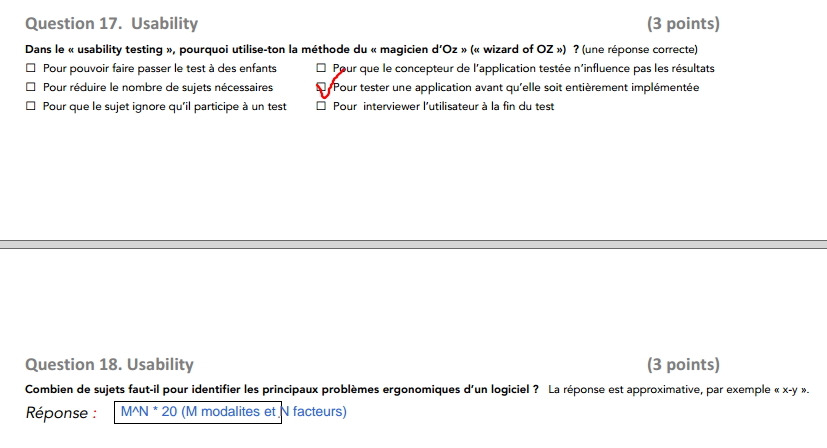
\includegraphics[scale=0.55]{./images/exercise4.png}
}
\end{figure}
































